\chapter{Background}\label{chap:background}
%\section{Introduction to Planning}
Planning in \acf{AI} is a fundamental aspect in the field that allows agents to formulate sequences of actions and strategies
to achieve a specific goal. It is used in a wide range of fields where agents need to make decisions and take actions based on the current state of the environment

Classical planning is a type of planning that is used in \ac{AI} to solve problems that can be represented as a set of states and actions.
It deals with straightforward actions \& with predictable and deterministic environments, where the agent can predict the outcome of its actions.
The challenge in classical planning is to construct a sequence of actions that will transform the initial state
of the environment into a desired goal state, while dealing with exponential growth in the search space, and dealing with the
actions and steps in chronological order.

Among the different types of planning, we have \textbf{state space planning} %, which is a type of planning that is used in \ac{AI} to solve problems searching through a set of states and actions,
and \textbf{plan space planning}. (They will be discussed in more details in the Key Definition section \ref{sec:key_definitions}) %, which is a type of planning that is used in \ac{AI} to solve problems searching through a set of partial plans and actions. 
In this thesis, we will focus on plan space planning, and more specifically on \acf{POP}.

Unity3D is a powerful game engine that is used to develop games, simulations, and virtual reality applications. It provides a lot of tools and features that can be used to create interactive and immersive experiences. \ac{VR} is a type of simulation that is used to create a virtual environment for the user.

In this chapter, we will start by providing some key definitions and concepts that are important to understand the \ac{POP} algorithm. Then, we will provide an overview of the \ac{POP} algorithm, the Unity3D game engine, and the applications of \ac{VR} and how it can be used to visualize the \ac{POP} algorithm.


%-----------------------------------------------------------------------------------------------------------------------------------



\section{Key Definitions and Concepts}\label{sec:key_definitions}
Here we will tackle some key definitions and concepts that are essential to understand the \ac{POP} algorithm.
All definitions and concepts in this section are based on the book "Artificial Intelligence: A Modern Approach" by Stuart Russell and Peter Norvig \cite{RN2020}, the book "Automated Planning: Theory \& Practice" by Malik Ghallab et al. \cite{10.5555/975615}, and on the lecture slides of the course "Introduction to Artificial Intelligence" by Prof. Haythem Ismail at the German University in Cairo \cite{Ismail2023}.
Now, in the following list, we will look at some key definitions and concepts in the field of planning:
% list of definitions
\begin{itemize}
    \item \textbf{Agent}: An Agent is an entity that can perceive its environment, make decisions, and take actions to achieve a specific goal. An agent can be a robot, a computer program, or a human being. It can be a simple agent that follows a set of rules, or it can be a complex agent that uses \ac{AI} to learn and adapt to its environment. For example, a self-driving car is an agent that uses sensors to perceive its environment, a specialized robot is an agent that can sense the environment and perform the required steps to achieve a specific goal.

    \item \textbf{State}: A State is a snapshot of the environment at a specific point in time. It represents the current configuration of the environment, including the location of objects, the status of objects, and the relationships between objects. In planning contexts, it can be represented as a set of propositions. For example, consider a robot that needs to navigate through a maze. The state of the robot can be represented as the location of the robot in the maze, the location of the walls, the location of the obstacles, and the location of the goal. The state of the robot changes as the robot moves through the maze, and the robot needs to update its state to reflect the changes in the environment.

    \item \label{def:state_space_planning}
          \textbf{State Space Planning}: State Space Planning is a type of planning that is used in \ac{AI} to solve problems searching through a set of states and actions. In this type of planning, the world is represented as a set of states, and the agent can move from one state to another by applying actions. While the agent is searching, it represents the world as a graph, where the nodes are states and the edges are actions. It has the ability to expand any node using the available actions, and it can backtrack if it reaches a dead-end. When the agent reaches any node, it runs a goal test to check if the current state is the goal state. If the goal test is successful, the agent stops and returns the solution. If the goal test fails, the agent continues searching and expanding until it finds a solution.

          For example, consider a robot that needs to pick up a package from one location and deliver it to another location. The robot can represent the world as a set of states, where the initial state that the robot is $At(location_A)$, and the goal state is to satisfy the condition Delivered($package, location_B$). The robot can move from one state to another by applying actions like Move($location_A$, $location_B$) and Pickup($package$, $location_C$) and Deliver($package$, $location_B$). Of course, there are some constraints and preconditions that the robot needs to satisfy before applying any action. For example, the robot cannot deliver a package if it has not picked it up first, and the robot cannot pick up a package from a location if the robot is not at that location. One way to solve this problem is to start from the goal state and work backward to the initial state, applying the actions in reverse order, and this is called backward state space planning. To achieve Delivered($package$, $location_B$), the robot needs to Deliver($package$, $location_B$), and to deliver the package, the robot needs to Pickup($package$, $location_C$) \& Move($Location_C$, $Location_B$), and to pick up the package, the robot needs to Move($location_A$, $location_C$). So, the robot needs to apply the actions Move($location_A$, $location_C$), Pickup($package$, $location_C$), Move($Location_C$, $Location_B$), and Deliver($package$, $location_B$) in this order to achieve the goal state Delivered($package$, $location_B$).

    \item \label{def:total_order_plan}
          \textbf{Total-Order Plan}: A Total-Order Plan is a plan that specifies a total order of actions. This means that it gives you a specific sequence of actions that need to be executed in a specific and strict order to achieve a specific goal. It does not give you the freedom or choices while executing the actions. For example, \textit{LeftSock}() $\rightarrow$ \textit{RightSock}() $\rightarrow$ \textit{LeftShoe}() $\rightarrow$ \textit{RightShoe}(), is a total-order plan that specifies a strict order to achieve \textit{wearing both shoes}. Other valid solutions may involve interchanging the order of the socks or the shoes as long as the socks are worn before the shoes. In \autoref{fig:socks_shoes_total_order_plan}, we can see 6 different total-order plans and each one of them can be considered a linearization of the partial order plan in \autoref{fig:socks_shoes_partial_order_plan}.
          \begin{figure}[ht]
              \centering

              \begin{tikzpicture}[node distance=1cm and 1cm, auto]

                  % Total-Order Plans
                  % You can replicate the structure below for each total-order plan
                  \node [rectangle,draw] (start1) {Start};
                  \node [below=of start1, rectangle,draw] (lsock1) {Left Sock};
                  \node [below=of lsock1, rectangle,draw] (rsock1) {Right Sock};
                  \node [below=of rsock1, rectangle,draw] (lshoe1) {Left Shoe};
                  \node [below=of lshoe1, rectangle,draw] (rshoe1) {Right Shoe};
                  \node [below=of rshoe1, rectangle,draw] (finish1) {Finish};

                  \draw[->] (start1) -- (lsock1);
                  \draw[->] (lsock1) -- (rsock1);
                  \draw[->] (rsock1) -- (lshoe1);
                  \draw[->] (lshoe1) -- (rshoe1);
                  \draw[->] (rshoe1) -- (finish1);

                  % Total-Order Plan 2
                  \node[right=1.5cm of start1, rectangle,draw] (start2) {Start};
                  \node [below=of start2, rectangle,draw] (lsock2) {Left Sock};
                  \node [below=of lsock2, rectangle,draw] (lshoe2) {Left Shoe};
                  \node [below=of lshoe2, rectangle,draw] (rsock2) {Right Sock};
                  \node [below=of rsock2, rectangle,draw] (rshoe2) {Right Shoe};
                  \node [below=of rshoe2, rectangle,draw] (finish2) {Finish};

                  \draw[->] (start2) -- (lsock2);
                  \draw[->] (lsock2) -- (lshoe2);
                  \draw[->] (lshoe2) -- (rsock2);
                  \draw[->] (rsock2) -- (rshoe2);
                  \draw[->] (rshoe2) -- (finish2);

                  % Total-Order Plan 3
                  \node[right=1.5cm of start2, rectangle,draw] (start3) {Start};
                  \node [below=of start3, rectangle,draw] (rsock3) {Right Sock};
                  \node [below=of rsock3, rectangle,draw] (lsock3) {Left Sock};
                  \node [below=of lsock3, rectangle,draw] (rshoe3) {Right Shoe};
                  \node [below=of rshoe3, rectangle,draw] (lshoe3) {Left Shoe};
                  \node [below=of lshoe3, rectangle,draw] (finish3) {Finish};

                  \draw[->] (start3) -- (rsock3);
                  \draw[->] (rsock3) -- (lsock3);
                  \draw[->] (lsock3) -- (rshoe3);
                  \draw[->] (rshoe3) -- (lshoe3);
                  \draw[->] (lshoe3) -- (finish3);

                  % Total-Order Plan 4
                  \node[right=1.5cm of start3, rectangle,draw] (start4) {Start};
                  \node [below=of start4, rectangle,draw] (rsock4) {Right Sock};
                  \node [below=of rsock4, rectangle,draw] (rshoe4) {Right Shoe};
                  \node [below=of rshoe4, rectangle,draw] (lsock4) {Left Sock};
                  \node [below=of lsock4, rectangle,draw] (lshoe4) {Left Shoe};
                  \node [below=of lshoe4, rectangle,draw] (finish4) {Finish};

                  \draw[->] (start4) -- (rsock4);
                  \draw[->] (rsock4) -- (rshoe4);
                  \draw[->] (rshoe4) -- (lsock4);
                  \draw[->] (lsock4) -- (lshoe4);
                  \draw[->] (lshoe4) -- (finish4);

                  % Total-Order Plan 5
                  \node[right=1.5cm of start4, rectangle,draw] (start5) {Start};
                  \node [below=of start5, rectangle,draw] (rsock5) {Right Sock};
                  \node [below=of rsock5, rectangle,draw] (lsock5) {Left Sock};
                  \node [below=of lsock5, rectangle,draw] (lshoe5) {Left Shoe};
                  \node [below=of lshoe5, rectangle,draw] (rshoe5) {Right Shoe};
                  \node [below=of rshoe5, rectangle,draw] (finish5) {Finish};

                  \draw[->] (start5) -- (rsock5);
                  \draw[->] (rsock5) -- (lsock5);
                  \draw[->] (lsock5) -- (lshoe5);
                  \draw[->] (lshoe5) -- (rshoe5);
                  \draw[->] (rshoe5) -- (finish5);

                  % Total-Order Plan 6
                  \node[right=1.5cm of start5, rectangle,draw] (start6) {Start};
                  \node [below=of start6, rectangle,draw] (lsock6) {Left Sock};
                  \node [below=of lsock6, rectangle,draw] (rsock6) {Right Sock};
                  \node [below=of rsock6, rectangle,draw] (rshoe6) {Right Shoe};
                  \node [below=of rshoe6, rectangle,draw] (lshoe6) {Left Shoe};
                  \node [below=of lshoe6, rectangle,draw] (finish6) {Finish};

                  \draw[->] (start6) -- (lsock6);
                  \draw[->] (lsock6) -- (rsock6);
                  \draw[->] (rsock6) -- (rshoe6);
                  \draw[->] (rshoe6) -- (lshoe6);
                  \draw[->] (lshoe6) -- (finish6);

              \end{tikzpicture}
              \caption{\centering Socks \& Shoes Total Order Plan solutions.}
              \label{fig:socks_shoes_total_order_plan}
          \end{figure}

    \item \label{def:partial_order_plan}
          \textbf{Partial-Order Plan}: A Partial-Order-Plan is a plan that does not specify a total order of actions, but instead specifies a partial order of actions. This means that it gives you a general structure of what needs to be done with some constraints and ordering between them, but some steps/actions are not given a specific order. This gives the agent the freedom to execute some actions in any order, as long as the constraints \& general structure are satisfied. For example, consider the problem of putting on socks and shoes. The general structure is to put on the socks first, then the shoes. But, the order in which you put on the left and right sock and shoe can vary. One person might put on the left sock first, then the right sock, then the left shoe, and finally the right shoe. Another person might interchange the order of the 2 socks or the 2 shoes, and so on. The partial plan does not specify the actual order of the final actions. (See \autoref{fig:socks_shoes_partial_order_plan})

          \begin{figure}[ht]
              \centering
              \begin{tikzpicture}[node distance=1cm and 1cm, auto]
                  % Partial-Order Plan
                  \node[rectangle,draw] (start) {Start};
                  \node[below left=of start, rectangle,draw] (lsock) {Left Sock};
                  \node[below right=of start, rectangle,draw] (rsock) {Right Sock};
                  \node[below=of lsock, rectangle,draw] (lshoe) {Left Shoe};
                  \node[below=of rsock, rectangle,draw] (rshoe) {Right Shoe};
                  \node[below=of $(lshoe)!0.5!(rshoe)$, rectangle,draw] (finish) {Finish};

                  \draw[->] (start) -- (lsock);
                  \draw[->] (start) -- (rsock);
                  \draw[->] (lsock) -- (lshoe);
                  \draw[->] (rsock) -- (rshoe);
                  \draw[->] (lshoe) -- (finish);
                  \draw[->] (rshoe) -- (finish);
              \end{tikzpicture}
              \caption{Socks \& Shoes Partial Order Plan solution.}
              \label{fig:socks_shoes_partial_order_plan}
          \end{figure}
    \item \label{def:plan_space_planning}
          \textbf{Plan Space Planning}: Plan Space Planning is a type of planning that is used in \ac{AI} to solve problems searching through a set of partial plans and actions. In this type of planning, the world is represented as some nodes, each node represents a partial plan, and the edges represent the actions that can be applied to move from one partial plan to another. The agent can explore the search space by expanding the nodes and applying the actions, can also backtrack, and it can explore multiple paths in parallel. The agent can also use problem decomposition to break down the problem into smaller subproblems, solve them independently, and then merge the subplans into a final plan. For example, consider the problem of cooking a meal. The agent can represent the world as a set of partial plans, where each partial plan represents a step in the cooking process. The agent can explore the search space by expanding the partial plans and applying the actions to move from one partial plan to another. The agent can use problem decomposition to break down the cooking process into smaller subproblems, such as chopping vegetables, boiling water, and frying meat. The agent can solve each subproblem independently and then merge the subplans into a final plan to cook the meal.

    \item \label{def:least_commitment_strategy}
          \textbf{Least Commitment Strategy}: Least Commitment Strategy is a strategy that does not require the planner to commit to a specific order of actions. Instead, the planner can choose to leave some actions unordered, and the planner can choose to order actions only when necessary. This allows the planner to explore a larger space of possible plans, and it allows the planner to find plans that are more flexible and more robust.

    \item \label{def:operator}
          \textbf{Operator}: An Operator is a tuple $o = (name, preconds, effects)$ where:
          \begin{itemize}
              \item $name$ is the name of the operator.
              \item $preconds$ is a set of preconditions that need to be satisfied before applying the operator.
              \item $effects$ is a set of effects that will be achieved after applying the operator.
          \end{itemize}
          Example: $Buy(item,store)$, $preconds = \{At(store)\}$, $effects = \{Has(item)\}$.

    \item \label{def:action}
          \textbf{Action}: An Action  is a partially instantiated operator,
          (i.e. any ground instance of an operator with some of its variables instantiated).
          Example: $Buy(item,store)$, $Buy(Oranges,Market)$, $Buy(Phone,store)$, are all actions.

    \item \label{def:achiever}
          \textbf{Achiever}: An Achiever is an operator that can achieve a specific precondition. For example, if we have a precondition $p_j$ that needs to be satisfied, the achiever of $p_j$ is an operator that has $p_j$ in its effects, and their \ac{MGU} is consistent with the bindings in the plan.

    \item \label{def:causal_link}
          \textbf{Causal Link}: A Causal Link is in the form of $(a_i \xrightarrow{\text{$P_j$}} a_j)$ where:
          \begin{itemize}
              \item $a_i$ is an action.
              \item $a_j$ is another action linked to $a_i$.
              \item $P_j$ is a precondition of $a_j$, and at the same time an effect of $a_i$.
          \end{itemize}
          An action $a_i$ is said to achieve a precondition $p_j$ if $p_j \in$ effects($a_i$) and $p_j \in$ preconds($a_j$).
          A causal link is initiated to ensure that there is another action, before the action with this precondition, that can satisfy it.
          \\ Example: $Go(store)$ $\xrightarrow{\text{$At(store)$}}$ $Buy(item,store)$, where $Go(store)$ achieves the precondition $At(store)$ for the action $Buy(item,store)$.

    \item \label{def:binding_constraint}
          \textbf{Binding Constraints}: Binding Constraints is a set of constraints that bind variables to values.
          For example, if we have a binding $B = \{x \leftarrow \{1,5\}, y \leftarrow 2\}$, this means that the variable $x$ is bound to the values 1 or 5,
          and the variable $y$ is bound to the value 2.

    \item \label{def:planning_problem}
          \textbf{Planning Problem}: A Planning Problem is a problem that can be represented as a set of states and actions. The goal of the planning problem is to find a sequence of actions that will transform the initial state of the environment into a desired goal state. The planning problem can be solved using classical planning algorithms, such as state space planning and plan space planning. A planning problem can be represented as a tuple $P = (O, s_0, g)$ \cite{10.5555/975615} where:
          \begin{itemize}
              \item $O$ is a set of operators.
              \item $s_0$ is the initial state.
              \item $g$ is the goal state.
          \end{itemize}
          Example: $Problem =$ (
          \begin{itemize}
              \item Operators: \{$Buy(item,store)$, $Go(somewhere)$\}
              \item Initial State: \{$At(Home)$\}
              \item Goal State: \{$Has$($Oranges$), $At(Home)$\}
          \end{itemize}
          ).\\
          This planning problem represents a simple problem where the agent needs to buy some oranges from the store and go back home.

    \item  \label{def:ordering_constraint}
          \textbf{Ordering Constraint ($\prec$)}: An Ordering Constraint is a constraint that specifies the order of actions in a partial order plan. It is in the form of $a_i \prec a_j$, which means that action $a_i$ must be executed before action $a_j$. The ordering constraint is used to ensure that the actions are executed in the correct order and to prevent conflicts between actions.

    \item  \label{def:partial_plan}
          \textbf{Partial Plan}: A Partial Plan is a tuple $\pi = (A, \prec, B, L)$ where:
          \begin{itemize}
              \item $A$ is a set of actions, or partially instantiated Operators.
              \item $\prec$ is a set of ordering constraints between actions in the form of $a_i \prec a_j$
              \item $B$ is a set of bindings.
              \item $L$ is a set of causal links.
          \end{itemize}
          are the components of a partial plan.


    \item  \label{def:consistency_partial_plan}
          \textbf{Consistency of Partial Plans}: A partial order plan $\pi = (A, \prec, B, L)$ is consistent if it satisfies the following conditions: \cite{10.5555/975615}
          \begin{itemize}
              \item The transitive closure of the ordering constraints $\prec$ is a strict partial order.
              \item every substitution $\sigma $ which binds a variable $x$ to a value in its allowed domain $D_x$ is consistent with the bindings in all other constraints in $B$.
          \end{itemize}


    \item  \label{def:threat}
          \textbf{Threat}: A Threat in a partial plan is an action that could potentially undo the effects of another action. A threat is a potential problem in a partial plan that needs to be resolved to make the plan consistent. An action $a_k$ threatens a causal link $(a_i \xrightarrow{\text{$P_j$}}  a_j)$ if it has the following properties:
          \begin{itemize}
              \item $e_k (\in$ effect of $a_k)$ unifies with $\lnot p_j$.
              \item the \ac{MGU} of $e_k$ and $\lnot p_j$ is consistent with the bindings in $B$.
              \item $\prec \cup \{a_i \prec a_k, a_k \prec a_j\}$ is consistent.
          \end{itemize}
          Once the 3 conditions are met, we can say that $a_k$ threatens the causal link $(a_i \xrightarrow{\text{$P_j$}}  a_j)$.
          Example: $Go(Cinema)$ threatens the causal link $(Go(Store) \xrightarrow{\text{$At(Store)$}} Buy(Oranges,Store))$, as it can negate the effect of being $At(Store)$.

    \item  \label{def:partial_plan_completion}
          \textbf{Partial Plan Completion}: A partial plan $\pi = (A, \prec, B, L)$ is complete if all the preconditions of the operators or actions in $A$ are satisfied and causally linked, and all causal links in $L$ are not threatened by any action in $A$.

\end{itemize}








\section{Partial Order Planning} \label{sec:partial_order_planning}
\acf{POP} is a plan-space search algorithm (See definition in Section \ref{def:plan_space_planning}) that searches through a set of partial plans.
Unlike other planning algorithms, \ac{POP} gives partial-ordered plans, which means that it does not specify a total order of actions.
This gives it the advantage over total order planning algorithms that it can use problem decomposition, work
on several subproblems in parallel independently, solve them with several subplans, and then merge the subplans into a final plan.


\ac{POP} uses least commitment strategy that does not require the planner to commit to a specific order of actions, as defined in Section \ref{def:least_commitment_strategy}. In addition, \ac{POP} uses closed-world assumption, which means that the planner assumes that everything that is not known or not stated is false. This allows the planner to make assumptions about the world and to make decisions based on the available information.
\ac{POP} is also sometimes represented as a \acf{DAG}, where the nodes represent actions, and the edges represent the causal links or the ordering constraints between actions. (See \autoref{fig:socks_shoes_partial_order_plan} for an example of a \ac{DAG} representing a partial order plan).

\subsection{POP Algorithm} \label{subsec:pop_algorithm}
The \acf{POP} algorithm works by incrementally building a partial order plan, and then refining the plan by adding operators, ordering constraints,
bindings, and causal links to resolve threats and make the plan consistent.
The planner keeps track of a set of pairs $(a_i, p_i)$, under the name of $agenda$, where $a_i$ is an action and $p_i$ is a precondition of $a_i$. The $agenda$ is used to keep track of the unsatisfied preconditions in the plan.


% POP Algorithm
\begin{algorithm}
    \caption{POP Algorithm}
    \label{alg:pop}
    \begin{algorithmic}[1]
        \STATE \textbf{Function} POP($O$, $s_0$, $g$)
        \ENSURE a plan
        \RETURN POP1($\{a_0, a_{\infty}\}, \{a_0 \prec a_{\infty}\}, \emptyset, \emptyset$, $\{a_{\infty}\} \times$ Preconds$(a_{\infty})$)\\

        \STATE --------------------------------------------------------------------------------
        %\hrule
        \STATE

        \STATE \textbf{Function} POP1($\pi = (A, L, \prec, B)$, agenda)
        \ENSURE a plan
        \IF{agenda == $\emptyset$}
        \RETURN $\pi$
        \ENDIF
        \STATE Select any pair $(a_i, p_i)$ and remove it from agenda
        \STATE achievers $\leftarrow$ the set of operators achieving $(a_i, p_i)$
        \IF{achievers == $\emptyset$}
        \RETURN $failure$
        \ENDIF
        \STATE \textcolor{red}{\textbf{\textit{Nondeterministically}}} choose some operator $a_j \in$ achievers
        \STATE $L \leftarrow L \cup \{\langle a_j \xrightarrow{\text{$P_i$}} a_i\rangle\}$
        \STATE Update $\prec$ with $a_j \xrightarrow{\text{$P_i$}} a_i$
        \STATE Update B with binding constraints of this link
        \IF{$a_j \notin A$}
        \STATE $A \leftarrow A \cup \{a_j\}$
        \STATE Update $\prec$ with $a_0 \prec a_j$ and $a_j \prec a_{\infty}$
        \STATE agenda $\leftarrow$ agenda $\cup \{(a_j, p_j)|p_j \in$ preconds$(a_j)\}$
        \ENDIF
        \STATE $\pi \leftarrow$ RESOLVE-THREATS($\pi$, $a_j$, $\langle a_j \prec a_i\rangle$)
        \RETURN POP1($\pi$, agenda)\\

        \STATE --------------------------------------------------------------------------------
        % \hrule
        \STATE

        \STATE \textbf{Function} RESOLVE-THREATS($\pi = (A, L, \prec, B)$, $a_l$, $L$)
        \ENSURE a plan
        \FOR{each threat $a_k$ on $(a_i \xrightarrow{\text{$P_j$}} a_j)$, where $a_k = a_l$ or $(a_i \xrightarrow{\text{$P_j$}} a_j) = l$}
        \STATE \textcolor{red}{\textbf{\textit{Nondeterministically}}} choose one of the following:
        \STATE - Update $\prec$ with $a_k \prec a_i$
        \STATE - Update with $a_j \prec a_k$
        \STATE - Add a binding constraint to $B$ which renders $p_i$ nonunifiable with any threatening effect of $a_k$.
        \ENDFOR
        \RETURN $\pi$
    \end{algorithmic}
\end{algorithm}

\subsubsection{Overview of the POP Algorithm Execution} \label{subsubsec:pop_execution}
The \ac{POP} algorithm starts by calling the POP function with the initial state $s_0$ and the goal state $g$, and some set of operators $O$. The POP function then initializes the plan with the initial and goal actions ($a_0$ \& $a_{\infty}$ respectively). The initial action (often referred to as Start) does not have any preconditions, just have effects, and these effects correspond to the initial state of the world. The goal action (often referred to as Finish) does not have any effects, just have preconditions, and these preconditions correspond to the goal state of the world (the conditions you need to meet to finish). Finally, the POP function initializes the agenda with the preconditions of the goal action $a_{\infty}$. For each precondition $p_i$ in the agenda, \textbf{$POP()$} adds the pair $(a_i, p_i)$ to the agenda.
Then the algorithm calls the POP1 function to start building the plan. The POP1 function selects any action from the agenda, randomly or based on some heuristic, then removes it from the agenda. It then finds the achievers of the selected action, and if there are no achievers, it returns a failure, as there are some condition that cannot be satisfied. If there are achievers, it nondeterministically chooses one of the achievers and adds it to the plan, as in line 14 of the algorithm \ref{alg:pop} (we will talk about nondeterminism in more details in \autoref{subsec:nondeterministic_achievers_threat_search}). It then updates the ordering constraints, bindings, and causal links in the plan in lines 15 to 17.
\textbf{$POP1()$} then checks if the selected action is already in the plan, if not, it does three things: adds the new action to the set of actions $A$, updates the ordering constraints with the new action to be ordered between the $Start$ and $Finish$ actions, and adds the preconditions of the new action to the agenda.
Finally, it resolves any threats in the plan in line 23 and calls the POP1 function recursively with the updated plan and agenda. The POP1 function continues to build the plan until the agenda is empty, at which point it returns the plan as the solution. If at any point the algorithm encounters a failure, it backtracks and tries a different path. The algorithm continues to explore the search space until it finds a valid plan or exhausts all possible paths.


\subsubsection{Threats Resolution} \label{subsubsec:threat_resolution}
Threats are potential problems in a partial plan that need to be resolved to make the plan consistent. A threat occurs when an action could potentially undo the effects of another action. The \ac{POP} algorithm uses a threat resolution mechanism to resolve threats and make the plan consistent. The algorithm checks for threats in the plan and resolves them by adding ordering constraints, bindings, or causal links to prevent the threat from occurring. The function \textbf{RESOLVE-THREATS} takes a partial plan $\pi = (A, L, \prec, B)$, an action $a_l$, and a causal link $L$ as input and resolves any threats in the plan.
The function gets any threat $a_k$ that threatens the causal link $L$, or any causal link that $a_l$ itself threatens. Letting $a_k$ be the action that threatens any of the causal links, and $link$ = $(a_i \xrightarrow{\text{$P_j$}} a_j)$ be the causal link that $a_k$ threatens, the function nondeterministically chooses one of the following options to resolve the threat: update the ordering constraints with $a_k \prec a_i$ (called \textbf{Demotion}), update with $a_j \prec a_k$ (called \textbf{Promotion}), or add a binding constraint to $B$ that renders $p_i$ nonunifiable with any threatening effect of $a_k$. The function then returns the updated plan with the resolved threats.
The threat resolution mechanism is an essential part of the \ac{POP} algorithm, as it ensures that the plan is consistent and that the actions are executed in the correct order.


\section{Unity 3D Engine} \label{sec:unity3d}
Unity is a cross-platform game engine developed by Unity Technologies. It was first announced and released in June 2005 at Apple Inc.'s Worldwide Developers Conference as a MacOS X-exclusive game engine \cite{WikiUnity}. The engine has since been gradually extended to support more than 25 platforms. It is used to create interactive 2D, 3D, \ac{VR}, and \ac{AR} applications. The engine can be used to create both three-dimensional and two-dimensional games as well as simulations for its many platforms. Unity's core advantages are its ease of use, and flexibility. Unity is a powerful engine that is used by developers around the world to create a wide range of games and applications.
One of the strongest features of Unity is its built-in physics engine, which allows developers to create realistic physics simulations in their games in a short amount of time.

\subsection{Virtual Reality} \label{subsec:virtual_reality}
\acf{VR} is a computer-generated simulation of an environment that can be interacted with in a seemingly real or physical way by a person using special electronic equipment \cite{WikiVR}. It has a wide range of applications. An important application of \ac{VR} is in the field of education and training. \ac{VR} was found effective in teaching complex subjects, such as engineering, medicine, and science. It allows students to interact with the subject in a more engaging and immersive way, which can help them better understand the concepts and principles behind the subject \cite{VRapps}\cite{WikiVR}.

\begin{figure}[H]
    \centering
    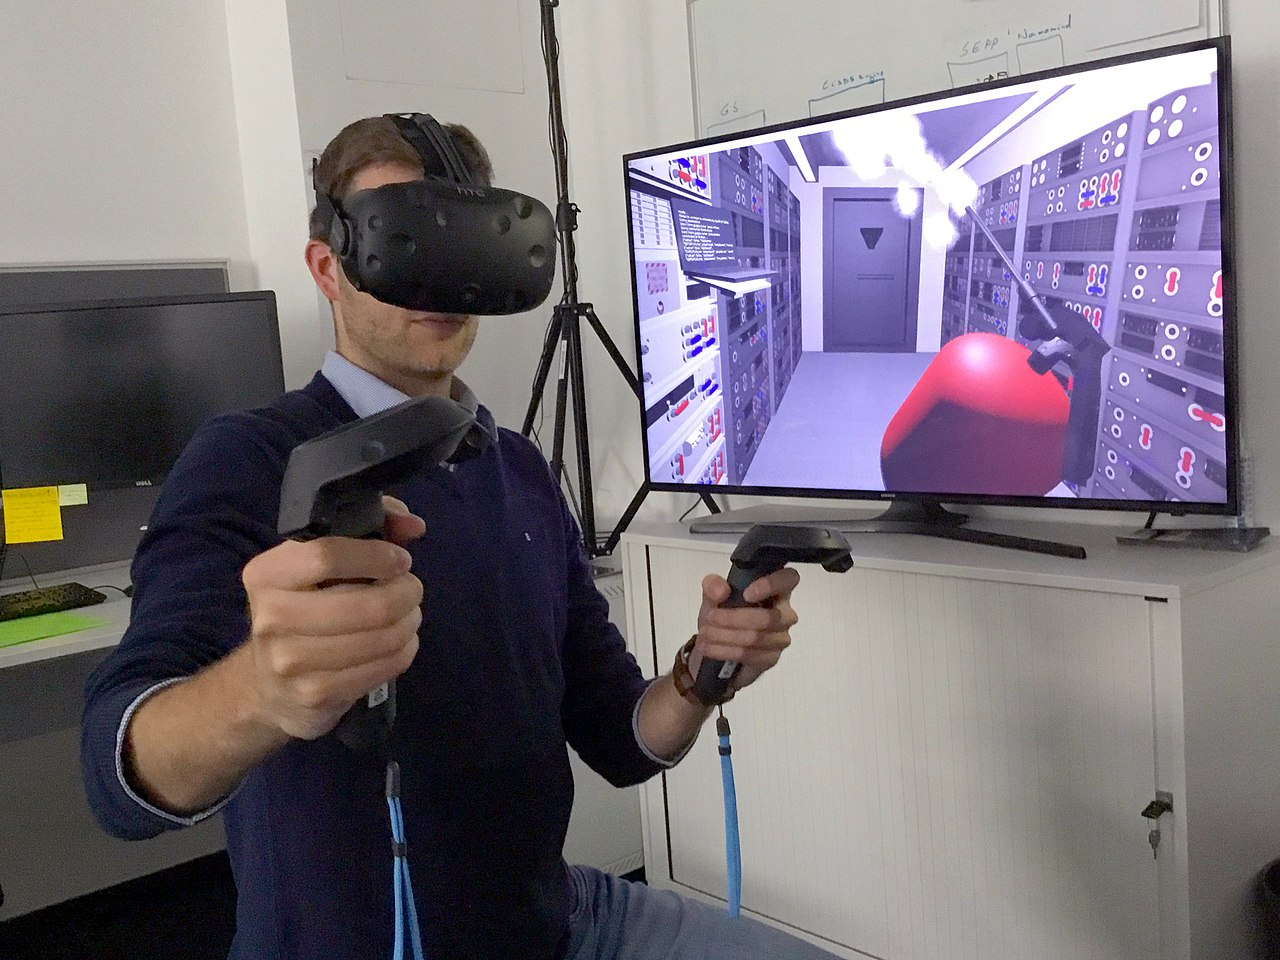
\includegraphics[width=0.4\textwidth]{images/VR.jpg}
    \caption{Virtual Reality in training and education. \cite{WikiVR}}
    \label{fig:vr_training}
\end{figure}


\subsection{\acf{VR} in Unity} \label{subsec:vr_in_unity}
Unity is a popular game engine that is used to create \ac{VR} applications. Unity provides a wide range of tools and features that make it easy to create \ac{VR} experiences. It supports a wide range of \ac{VR} devices, including the Oculus Rift, HTC Vive, and PlayStation \ac{VR}. It also provides a set of tools and APIs that make it easy to create \ac{VR} applications. Unity's \ac{VR} support includes features such as stereoscopic rendering, head tracking, and motion controllers.
\subsection{Visualization of the \acf{POP} Algorithm in Unity} \label{subsec:visualization_pop_unity}
In this thesis, Unity was used to visualize the \ac{POP} algorithm.
I created a 3D environment that represents the planning problem, and I used Unity's physics engine to simulate the actions and effects of the operators as a self arranging \ac{DAG} in the plan. I also used Unity's \ac{VR} support to create an immersive \ac{VR} experience that allows users to interact with the planning problem in a virtual environment. The goal of this visualization is to provide a more intuitive and interactive way to understand the \ac{POP} algorithm and how it works for new learners. By visualizing the algorithm in Unity, we hope to make it more accessible and engaging for users, and to help them better understand the concepts and principles behind the \ac{POP} algorithm.
